\documentclass[twoside]{book}

% Packages required by doxygen
\usepackage{fixltx2e}
\usepackage{calc}
\usepackage{doxygen}
\usepackage[export]{adjustbox} % also loads graphicx
\usepackage{graphicx}
\usepackage[utf8]{inputenc}
\usepackage{makeidx}
\usepackage{multicol}
\usepackage{multirow}
\PassOptionsToPackage{warn}{textcomp}
\usepackage{textcomp}
\usepackage[nointegrals]{wasysym}
\usepackage[table]{xcolor}

% Font selection
\usepackage[T1]{fontenc}
\usepackage[scaled=.90]{helvet}
\usepackage{courier}
\usepackage{amssymb}
\usepackage{sectsty}
\renewcommand{\familydefault}{\sfdefault}
\allsectionsfont{%
  \fontseries{bc}\selectfont%
  \color{darkgray}%
}
\renewcommand{\DoxyLabelFont}{%
  \fontseries{bc}\selectfont%
  \color{darkgray}%
}
\newcommand{\+}{\discretionary{\mbox{\scriptsize$\hookleftarrow$}}{}{}}

% Page & text layout
\usepackage{geometry}
\geometry{%
  a4paper,%
  top=2.5cm,%
  bottom=2.5cm,%
  left=2.5cm,%
  right=2.5cm%
}
\tolerance=750
\hfuzz=15pt
\hbadness=750
\setlength{\emergencystretch}{15pt}
\setlength{\parindent}{0cm}
\setlength{\parskip}{3ex plus 2ex minus 2ex}
\makeatletter
\renewcommand{\paragraph}{%
  \@startsection{paragraph}{4}{0ex}{-1.0ex}{1.0ex}{%
    \normalfont\normalsize\bfseries\SS@parafont%
  }%
}
\renewcommand{\subparagraph}{%
  \@startsection{subparagraph}{5}{0ex}{-1.0ex}{1.0ex}{%
    \normalfont\normalsize\bfseries\SS@subparafont%
  }%
}
\makeatother

% Headers & footers
\usepackage{fancyhdr}
\pagestyle{fancyplain}
\fancyhead[LE]{\fancyplain{}{\bfseries\thepage}}
\fancyhead[CE]{\fancyplain{}{}}
\fancyhead[RE]{\fancyplain{}{\bfseries\leftmark}}
\fancyhead[LO]{\fancyplain{}{\bfseries\rightmark}}
\fancyhead[CO]{\fancyplain{}{}}
\fancyhead[RO]{\fancyplain{}{\bfseries\thepage}}
\fancyfoot[LE]{\fancyplain{}{}}
\fancyfoot[CE]{\fancyplain{}{}}
\fancyfoot[RE]{\fancyplain{}{\bfseries\scriptsize Generated by Doxygen }}
\fancyfoot[LO]{\fancyplain{}{\bfseries\scriptsize Generated by Doxygen }}
\fancyfoot[CO]{\fancyplain{}{}}
\fancyfoot[RO]{\fancyplain{}{}}
\renewcommand{\footrulewidth}{0.4pt}
\renewcommand{\chaptermark}[1]{%
  \markboth{#1}{}%
}
\renewcommand{\sectionmark}[1]{%
  \markright{\thesection\ #1}%
}

% Indices & bibliography
\usepackage{natbib}
\usepackage[titles]{tocloft}
\setcounter{tocdepth}{3}
\setcounter{secnumdepth}{5}
\makeindex

% Hyperlinks (required, but should be loaded last)
\usepackage{ifpdf}
\ifpdf
  \usepackage[pdftex,pagebackref=true]{hyperref}
\else
  \usepackage[ps2pdf,pagebackref=true]{hyperref}
\fi
\hypersetup{%
  colorlinks=true,%
  linkcolor=blue,%
  citecolor=blue,%
  unicode%
}

% Custom commands
\newcommand{\clearemptydoublepage}{%
  \newpage{\pagestyle{empty}\cleardoublepage}%
}

\usepackage{caption}
\captionsetup{labelsep=space,justification=centering,font={bf},singlelinecheck=off,skip=4pt,position=top}

%===== C O N T E N T S =====

\begin{document}

% Titlepage & ToC
\hypersetup{pageanchor=false,
             bookmarksnumbered=true,
             pdfencoding=unicode
            }
\pagenumbering{alph}
\begin{titlepage}
\vspace*{7cm}
\begin{center}%
{\Large Project 2 }\\
\vspace*{1cm}
{\large Generated by Doxygen 1.8.13}\\
\end{center}
\end{titlepage}
\clearemptydoublepage
\pagenumbering{roman}
\tableofcontents
\clearemptydoublepage
\pagenumbering{arabic}
\hypersetup{pageanchor=true}

%--- Begin generated contents ---
\chapter{Hierarchical Index}
\section{Class Hierarchy}
This inheritance list is sorted roughly, but not completely, alphabetically\+:\begin{DoxyCompactList}
\item \contentsline{section}{Dornx3}{\pageref{class_dornx3}}{}
\begin{DoxyCompactList}
\item \contentsline{section}{Dornx2}{\pageref{class_dornx2}}{}
\end{DoxyCompactList}
\item \contentsline{section}{Inputs}{\pageref{struct_inputs}}{}
\item \contentsline{section}{Play}{\pageref{class_play}}{}
\begin{DoxyCompactList}
\item \contentsline{section}{Again}{\pageref{class_again}}{}
\end{DoxyCompactList}
\end{DoxyCompactList}

\chapter{Class Index}
\section{Class List}
Here are the classes, structs, unions and interfaces with brief descriptions\+:\begin{DoxyCompactList}
\item\contentsline{section}{\hyperlink{struct_inputs}{Inputs} }{\pageref{struct_inputs}}{}
\end{DoxyCompactList}

\chapter{File Index}
\section{File List}
Here is a list of all files with brief descriptions\+:\begin{DoxyCompactList}
\item\contentsline{section}{\hyperlink{_8dep_8inc}{.\+dep.\+inc} }{\pageref{_8dep_8inc}}{}
\item\contentsline{section}{\hyperlink{main_8cpp}{main.\+cpp} }{\pageref{main_8cpp}}{}
\end{DoxyCompactList}

\chapter{Class Documentation}
\hypertarget{class_again}{}\section{Again Class Reference}
\label{class_again}\index{Again@{Again}}


{\ttfamily \#include $<$dornx2.\+h$>$}

Inheritance diagram for Again\+:\begin{figure}[H]
\begin{center}
\leavevmode
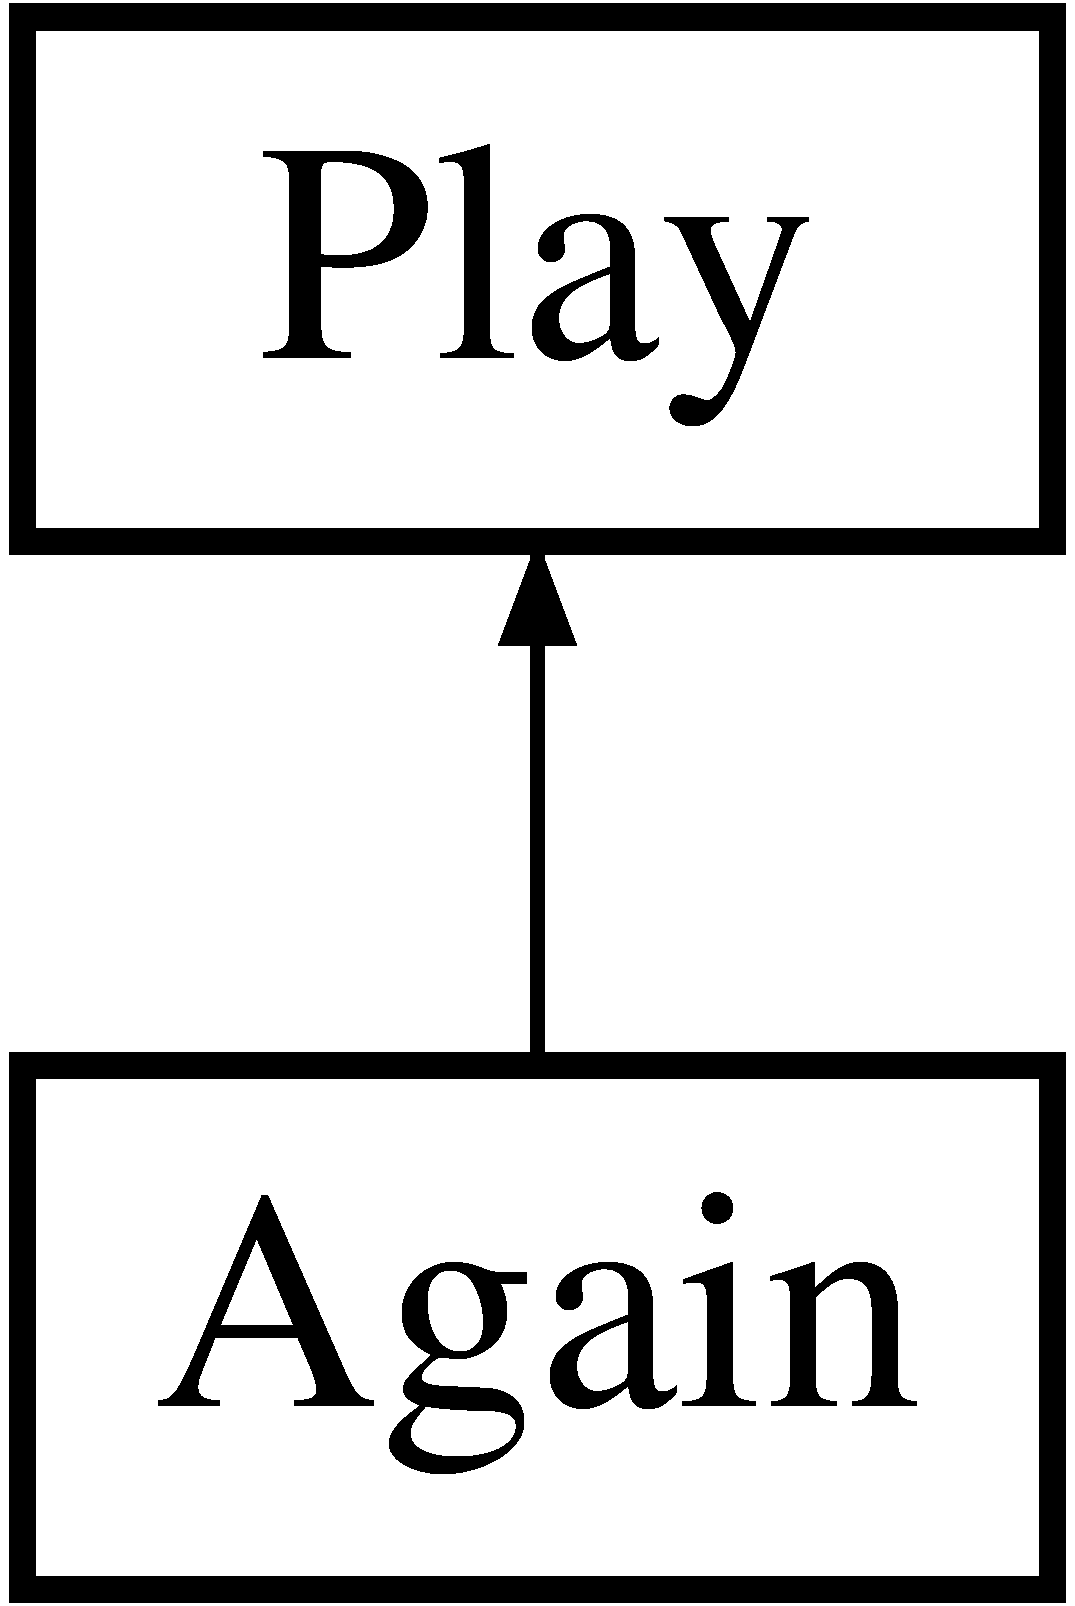
\includegraphics[height=2.000000cm]{class_again}
\end{center}
\end{figure}
\subsection*{Public Member Functions}
\begin{DoxyCompactItemize}
\item 
void \hyperlink{class_again_af3e99a5b59be21b644823ce7a9837a8f}{show} ()
\end{DoxyCompactItemize}


\subsection{Detailed Description}


Definition at line 38 of file dornx2.\+h.



\subsection{Member Function Documentation}
\mbox{\Hypertarget{class_again_af3e99a5b59be21b644823ce7a9837a8f}\label{class_again_af3e99a5b59be21b644823ce7a9837a8f}} 
\index{Again@{Again}!show@{show}}
\index{show@{show}!Again@{Again}}
\subsubsection{\texorpdfstring{show()}{show()}}
{\footnotesize\ttfamily void Again\+::show (\begin{DoxyParamCaption}{ }\end{DoxyParamCaption})\hspace{0.3cm}{\ttfamily [inline]}, {\ttfamily [virtual]}}



Reimplemented from \hyperlink{class_play_a87bb5456a9fcecfb9075b73db83d1e4c}{Play}.



Definition at line 40 of file dornx2.\+h.



The documentation for this class was generated from the following file\+:\begin{DoxyCompactItemize}
\item 
\hyperlink{dornx2_8h}{dornx2.\+h}\end{DoxyCompactItemize}

\hypertarget{class_dornx2}{}\section{Dornx2 Class Reference}
\label{class_dornx2}\index{Dornx2@{Dornx2}}


{\ttfamily \#include $<$dornx2.\+h$>$}

Inheritance diagram for Dornx2\+:\begin{figure}[H]
\begin{center}
\leavevmode
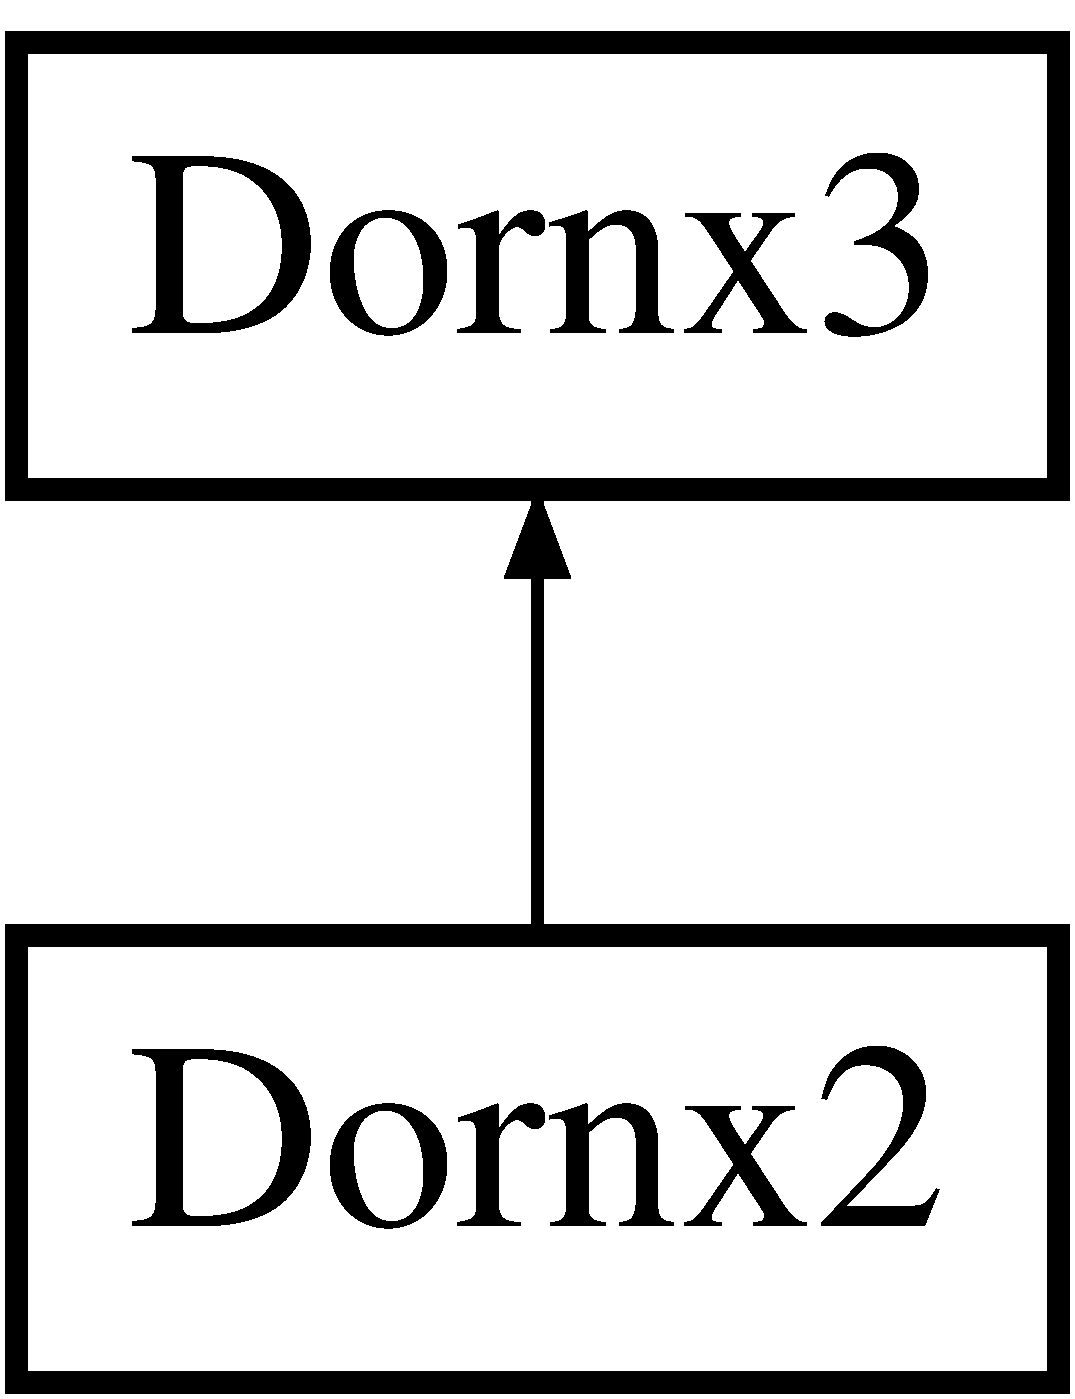
\includegraphics[height=2.000000cm]{class_dornx2}
\end{center}
\end{figure}
\subsection*{Public Member Functions}
\begin{DoxyCompactItemize}
\item 
virtual void \hyperlink{class_dornx2_a358fdbc837f4bc24f66980a7153babe3}{show} ()
\item 
void \hyperlink{class_dornx2_aa3fcfcbe016f42f136e105e58d58baf7}{dornx2} (float)
\item 
void \hyperlink{class_dornx2_abec89827e72c13b981b5fbd169234463}{dornx1} (float)
\item 
bool \hyperlink{class_dornx2_adf347547aec5c4ff26a6a6650d992062}{find\+Col} (string \mbox{[}$\,$\mbox{]}, int, string)
\end{DoxyCompactItemize}
\subsection*{Public Attributes}
\begin{DoxyCompactItemize}
\item 
float \hyperlink{class_dornx2_a625cb1bab8577b56ad9fdd30429b2cc1}{bet}
\item 
float \hyperlink{class_dornx2_a39b0aa95ebb2d298ce227e3052e9ee1f}{payout}
\item 
float \hyperlink{class_dornx2_a9721d2b992a38ebf38b3d9ba1106ac24}{sum} = 0
\item 
float \hyperlink{class_dornx2_a08c22beb426bb80169c29bd6fe382781}{pwings} = 0
\item 
float \hyperlink{class_dornx2_aeb5ee2bf43b55d212169fe6842c4dda0}{wins} = 0
\item 
float \hyperlink{class_dornx2_a901e60654dd16c22ab2f5bbf69e7ee47}{losses} = 0
\end{DoxyCompactItemize}


\subsection{Detailed Description}


Definition at line 17 of file dornx2.\+h.



\subsection{Member Function Documentation}
\mbox{\Hypertarget{class_dornx2_abec89827e72c13b981b5fbd169234463}\label{class_dornx2_abec89827e72c13b981b5fbd169234463}} 
\index{Dornx2@{Dornx2}!dornx1@{dornx1}}
\index{dornx1@{dornx1}!Dornx2@{Dornx2}}
\subsubsection{\texorpdfstring{dornx1()}{dornx1()}}
{\footnotesize\ttfamily void Dornx2\+::dornx1 (\begin{DoxyParamCaption}\item[{float}]{n }\end{DoxyParamCaption})}



Definition at line 23 of file dornx2f.\+cpp.

\mbox{\Hypertarget{class_dornx2_aa3fcfcbe016f42f136e105e58d58baf7}\label{class_dornx2_aa3fcfcbe016f42f136e105e58d58baf7}} 
\index{Dornx2@{Dornx2}!dornx2@{dornx2}}
\index{dornx2@{dornx2}!Dornx2@{Dornx2}}
\subsubsection{\texorpdfstring{dornx2()}{dornx2()}}
{\footnotesize\ttfamily void Dornx2\+::dornx2 (\begin{DoxyParamCaption}\item[{float}]{n }\end{DoxyParamCaption})}



Definition at line 39 of file dornx2f.\+cpp.

\mbox{\Hypertarget{class_dornx2_adf347547aec5c4ff26a6a6650d992062}\label{class_dornx2_adf347547aec5c4ff26a6a6650d992062}} 
\index{Dornx2@{Dornx2}!find\+Col@{find\+Col}}
\index{find\+Col@{find\+Col}!Dornx2@{Dornx2}}
\subsubsection{\texorpdfstring{find\+Col()}{findCol()}}
{\footnotesize\ttfamily bool Dornx2\+::find\+Col (\begin{DoxyParamCaption}\item[{string}]{\mbox{[}$\,$\mbox{]},  }\item[{int}]{,  }\item[{string}]{ }\end{DoxyParamCaption})}

\mbox{\Hypertarget{class_dornx2_a358fdbc837f4bc24f66980a7153babe3}\label{class_dornx2_a358fdbc837f4bc24f66980a7153babe3}} 
\index{Dornx2@{Dornx2}!show@{show}}
\index{show@{show}!Dornx2@{Dornx2}}
\subsubsection{\texorpdfstring{show()}{show()}}
{\footnotesize\ttfamily virtual void Dornx2\+::show (\begin{DoxyParamCaption}{ }\end{DoxyParamCaption})\hspace{0.3cm}{\ttfamily [inline]}, {\ttfamily [virtual]}}



Definition at line 25 of file dornx2.\+h.



\subsection{Member Data Documentation}
\mbox{\Hypertarget{class_dornx2_a625cb1bab8577b56ad9fdd30429b2cc1}\label{class_dornx2_a625cb1bab8577b56ad9fdd30429b2cc1}} 
\index{Dornx2@{Dornx2}!bet@{bet}}
\index{bet@{bet}!Dornx2@{Dornx2}}
\subsubsection{\texorpdfstring{bet}{bet}}
{\footnotesize\ttfamily float Dornx2\+::bet}



Definition at line 19 of file dornx2.\+h.

\mbox{\Hypertarget{class_dornx2_a901e60654dd16c22ab2f5bbf69e7ee47}\label{class_dornx2_a901e60654dd16c22ab2f5bbf69e7ee47}} 
\index{Dornx2@{Dornx2}!losses@{losses}}
\index{losses@{losses}!Dornx2@{Dornx2}}
\subsubsection{\texorpdfstring{losses}{losses}}
{\footnotesize\ttfamily float Dornx2\+::losses = 0}



Definition at line 24 of file dornx2.\+h.

\mbox{\Hypertarget{class_dornx2_a39b0aa95ebb2d298ce227e3052e9ee1f}\label{class_dornx2_a39b0aa95ebb2d298ce227e3052e9ee1f}} 
\index{Dornx2@{Dornx2}!payout@{payout}}
\index{payout@{payout}!Dornx2@{Dornx2}}
\subsubsection{\texorpdfstring{payout}{payout}}
{\footnotesize\ttfamily float Dornx2\+::payout}



Definition at line 20 of file dornx2.\+h.

\mbox{\Hypertarget{class_dornx2_a08c22beb426bb80169c29bd6fe382781}\label{class_dornx2_a08c22beb426bb80169c29bd6fe382781}} 
\index{Dornx2@{Dornx2}!pwings@{pwings}}
\index{pwings@{pwings}!Dornx2@{Dornx2}}
\subsubsection{\texorpdfstring{pwings}{pwings}}
{\footnotesize\ttfamily float Dornx2\+::pwings = 0}



Definition at line 22 of file dornx2.\+h.

\mbox{\Hypertarget{class_dornx2_a9721d2b992a38ebf38b3d9ba1106ac24}\label{class_dornx2_a9721d2b992a38ebf38b3d9ba1106ac24}} 
\index{Dornx2@{Dornx2}!sum@{sum}}
\index{sum@{sum}!Dornx2@{Dornx2}}
\subsubsection{\texorpdfstring{sum}{sum}}
{\footnotesize\ttfamily float Dornx2\+::sum = 0}



Definition at line 21 of file dornx2.\+h.

\mbox{\Hypertarget{class_dornx2_aeb5ee2bf43b55d212169fe6842c4dda0}\label{class_dornx2_aeb5ee2bf43b55d212169fe6842c4dda0}} 
\index{Dornx2@{Dornx2}!wins@{wins}}
\index{wins@{wins}!Dornx2@{Dornx2}}
\subsubsection{\texorpdfstring{wins}{wins}}
{\footnotesize\ttfamily float Dornx2\+::wins = 0}



Definition at line 23 of file dornx2.\+h.



The documentation for this class was generated from the following files\+:\begin{DoxyCompactItemize}
\item 
\hyperlink{dornx2_8h}{dornx2.\+h}\item 
\hyperlink{dornx2f_8cpp}{dornx2f.\+cpp}\end{DoxyCompactItemize}

\hypertarget{class_dornx3}{}\section{Dornx3 Class Reference}
\label{class_dornx3}\index{Dornx3@{Dornx3}}


{\ttfamily \#include $<$dornx3.\+h$>$}

Inheritance diagram for Dornx3\+:\begin{figure}[H]
\begin{center}
\leavevmode
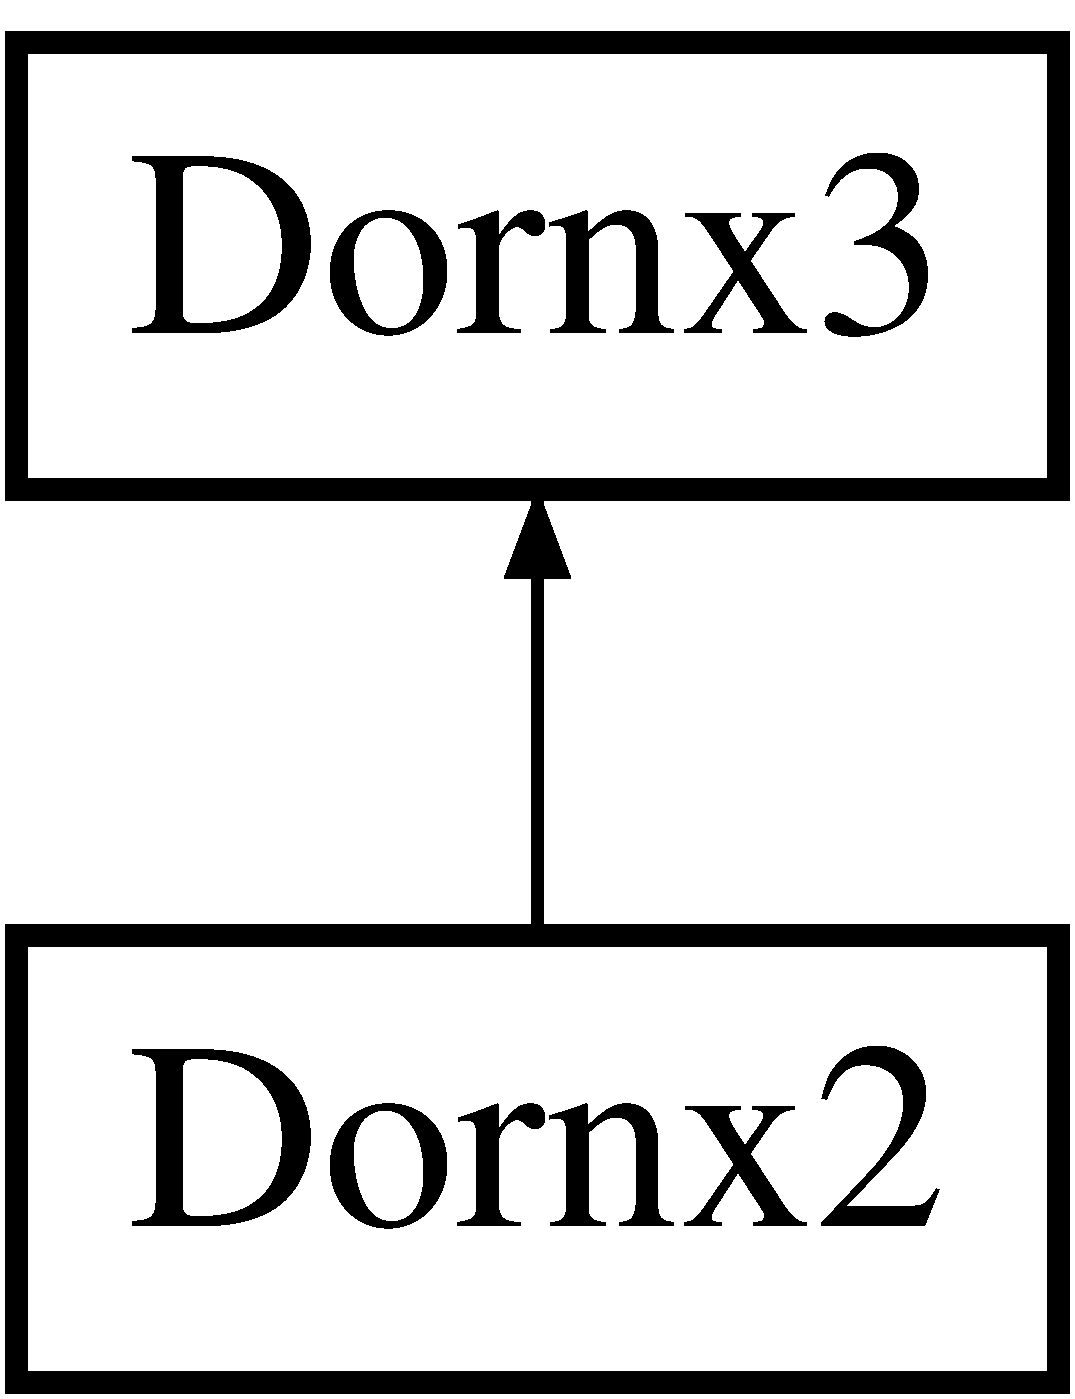
\includegraphics[height=2.000000cm]{class_dornx3}
\end{center}
\end{figure}
\subsection*{Public Attributes}
\begin{DoxyCompactItemize}
\item 
string \hyperlink{class_dornx3_aa8cbadbae14b2e9a29e38ba9b0ed37ba}{respond}
\item 
string \hyperlink{class_dornx3_ab2a8fd3713629e06177cf91b7221b82b}{bcolor}
\item 
string \hyperlink{class_dornx3_afb914249485c727f99503ac24e5b444f}{rcolor}
\item 
string \hyperlink{class_dornx3_a23ed936890f7aac31561df8819a5bb2e}{vcolor} \mbox{[}\hyperlink{dornx3_8h_abbca5f70b1b16867a3fd2f340a1fbdd9}{S\+I\+Z\+E2}\mbox{]} = \{\char`\"{}Red\char`\"{},\char`\"{}\hyperlink{class_dornx3_a556c86898a12bc10ff4a559d822cea1a}{red}\char`\"{},\char`\"{}R\+ED\char`\"{},\char`\"{}r\char`\"{},\char`\"{}Blue\char`\"{},\char`\"{}\hyperlink{class_dornx3_ad4294dbbc1608b76c5e49736b3bb8a86}{blue}\char`\"{}, \char`\"{}B\+L\+UE\char`\"{},\char`\"{}b\char`\"{}\}
\item 
string \hyperlink{class_dornx3_a556c86898a12bc10ff4a559d822cea1a}{red} \mbox{[}\hyperlink{dornx3_8h_afd1642892fe952b92046b3b290301c66}{C\+O\+L\+O\+R2}\mbox{]} = \{\char`\"{}Red\char`\"{},\char`\"{}red\char`\"{},\char`\"{}R\+ED\char`\"{},\char`\"{}r\char`\"{}\}
\item 
string \hyperlink{class_dornx3_ad4294dbbc1608b76c5e49736b3bb8a86}{blue} \mbox{[}\hyperlink{dornx3_8h_afd1642892fe952b92046b3b290301c66}{C\+O\+L\+O\+R2}\mbox{]} = \{\char`\"{}Blue\char`\"{},\char`\"{}blue\char`\"{},\char`\"{}B\+L\+UE\char`\"{},\char`\"{}b\char`\"{}\}
\end{DoxyCompactItemize}


\subsection{Detailed Description}


Definition at line 19 of file dornx3.\+h.



\subsection{Member Data Documentation}
\mbox{\Hypertarget{class_dornx3_ab2a8fd3713629e06177cf91b7221b82b}\label{class_dornx3_ab2a8fd3713629e06177cf91b7221b82b}} 
\index{Dornx3@{Dornx3}!bcolor@{bcolor}}
\index{bcolor@{bcolor}!Dornx3@{Dornx3}}
\subsubsection{\texorpdfstring{bcolor}{bcolor}}
{\footnotesize\ttfamily string Dornx3\+::bcolor}



Definition at line 22 of file dornx3.\+h.

\mbox{\Hypertarget{class_dornx3_ad4294dbbc1608b76c5e49736b3bb8a86}\label{class_dornx3_ad4294dbbc1608b76c5e49736b3bb8a86}} 
\index{Dornx3@{Dornx3}!blue@{blue}}
\index{blue@{blue}!Dornx3@{Dornx3}}
\subsubsection{\texorpdfstring{blue}{blue}}
{\footnotesize\ttfamily string Dornx3\+::blue\mbox{[}\hyperlink{dornx3_8h_afd1642892fe952b92046b3b290301c66}{C\+O\+L\+O\+R2}\mbox{]} = \{\char`\"{}Blue\char`\"{},\char`\"{}blue\char`\"{},\char`\"{}B\+L\+UE\char`\"{},\char`\"{}b\char`\"{}\}}



Definition at line 26 of file dornx3.\+h.

\mbox{\Hypertarget{class_dornx3_afb914249485c727f99503ac24e5b444f}\label{class_dornx3_afb914249485c727f99503ac24e5b444f}} 
\index{Dornx3@{Dornx3}!rcolor@{rcolor}}
\index{rcolor@{rcolor}!Dornx3@{Dornx3}}
\subsubsection{\texorpdfstring{rcolor}{rcolor}}
{\footnotesize\ttfamily string Dornx3\+::rcolor}



Definition at line 23 of file dornx3.\+h.

\mbox{\Hypertarget{class_dornx3_a556c86898a12bc10ff4a559d822cea1a}\label{class_dornx3_a556c86898a12bc10ff4a559d822cea1a}} 
\index{Dornx3@{Dornx3}!red@{red}}
\index{red@{red}!Dornx3@{Dornx3}}
\subsubsection{\texorpdfstring{red}{red}}
{\footnotesize\ttfamily string Dornx3\+::red\mbox{[}\hyperlink{dornx3_8h_afd1642892fe952b92046b3b290301c66}{C\+O\+L\+O\+R2}\mbox{]} = \{\char`\"{}Red\char`\"{},\char`\"{}red\char`\"{},\char`\"{}R\+ED\char`\"{},\char`\"{}r\char`\"{}\}}



Definition at line 25 of file dornx3.\+h.

\mbox{\Hypertarget{class_dornx3_aa8cbadbae14b2e9a29e38ba9b0ed37ba}\label{class_dornx3_aa8cbadbae14b2e9a29e38ba9b0ed37ba}} 
\index{Dornx3@{Dornx3}!respond@{respond}}
\index{respond@{respond}!Dornx3@{Dornx3}}
\subsubsection{\texorpdfstring{respond}{respond}}
{\footnotesize\ttfamily string Dornx3\+::respond}



Definition at line 21 of file dornx3.\+h.

\mbox{\Hypertarget{class_dornx3_a23ed936890f7aac31561df8819a5bb2e}\label{class_dornx3_a23ed936890f7aac31561df8819a5bb2e}} 
\index{Dornx3@{Dornx3}!vcolor@{vcolor}}
\index{vcolor@{vcolor}!Dornx3@{Dornx3}}
\subsubsection{\texorpdfstring{vcolor}{vcolor}}
{\footnotesize\ttfamily string Dornx3\+::vcolor\mbox{[}\hyperlink{dornx3_8h_abbca5f70b1b16867a3fd2f340a1fbdd9}{S\+I\+Z\+E2}\mbox{]} = \{\char`\"{}Red\char`\"{},\char`\"{}\hyperlink{class_dornx3_a556c86898a12bc10ff4a559d822cea1a}{red}\char`\"{},\char`\"{}R\+ED\char`\"{},\char`\"{}r\char`\"{},\char`\"{}Blue\char`\"{},\char`\"{}\hyperlink{class_dornx3_ad4294dbbc1608b76c5e49736b3bb8a86}{blue}\char`\"{}, \char`\"{}B\+L\+UE\char`\"{},\char`\"{}b\char`\"{}\}}



Definition at line 24 of file dornx3.\+h.



The documentation for this class was generated from the following file\+:\begin{DoxyCompactItemize}
\item 
\hyperlink{dornx3_8h}{dornx3.\+h}\end{DoxyCompactItemize}

\hypertarget{struct_inputs}{}\section{Inputs Struct Reference}
\label{struct_inputs}\index{Inputs@{Inputs}}
\subsection*{Public Attributes}
\begin{DoxyCompactItemize}
\item 
string \hyperlink{struct_inputs_a8c55eda886194176c889c08a30a669a6}{passwrd}
\item 
string \hyperlink{struct_inputs_a890a399e0575f0ab410e101f3748d04a}{usrname}
\item 
string \hyperlink{struct_inputs_a7a35f3dd65cc7f24cd3e4940bd36fa74}{bcolor}
\item 
string \hyperlink{struct_inputs_a3b8bbe1d2d8f1736d88f6130e800ac16}{rcolor}
\item 
float \hyperlink{struct_inputs_af2dd0562ce671279d010f1f6c927e719}{bet}
\item 
float \hyperlink{struct_inputs_ae019de875b0b547d9f6ff125068762c0}{payout}
\item 
float \hyperlink{struct_inputs_ab43ee7fc7282e8dadf5ae6d40453ccda}{sum} = 0
\item 
float \hyperlink{struct_inputs_a3ec027582343b553787b0e956a84bfae}{pwings} = 0
\item 
float \hyperlink{struct_inputs_a29b8137642d1269f9ef32b785200c17c}{wins} = 0
\item 
float \hyperlink{struct_inputs_a55580df8b5ddf655fc8f144ac1037863}{losses} = 0
\item 
string \hyperlink{struct_inputs_a80018d9bf94a9c6ea573b93ed30f89a6}{vcolor} \mbox{[}\hyperlink{main_8cpp_af08413a3ee12cf78b0ddeea71e2648b3}{S\+I\+ZE}\mbox{]} = \{\char`\"{}Red\char`\"{},\char`\"{}\hyperlink{struct_inputs_a7e6f084b57b2515a6d260d422b252f37}{red}\char`\"{},\char`\"{}R\+ED\char`\"{},\char`\"{}r\char`\"{},\char`\"{}Blue\char`\"{},\char`\"{}\hyperlink{struct_inputs_a685a6f5b41c965ecc2ff5ede529649da}{blue}\char`\"{}, \char`\"{}B\+L\+UE\char`\"{},\char`\"{}b\char`\"{}\}
\item 
string \hyperlink{struct_inputs_a7e6f084b57b2515a6d260d422b252f37}{red} \mbox{[}\hyperlink{main_8cpp_aa6d8034c897057de595a4511a4e7a837}{C\+O\+L\+OR}\mbox{]} = \{\char`\"{}Red\char`\"{},\char`\"{}red\char`\"{},\char`\"{}R\+ED\char`\"{},\char`\"{}r\char`\"{}\}
\item 
string \hyperlink{struct_inputs_a685a6f5b41c965ecc2ff5ede529649da}{blue} \mbox{[}\hyperlink{main_8cpp_aa6d8034c897057de595a4511a4e7a837}{C\+O\+L\+OR}\mbox{]} = \{\char`\"{}Blue\char`\"{},\char`\"{}blue\char`\"{},\char`\"{}B\+L\+UE\char`\"{},\char`\"{}b\char`\"{}\}
\item 
char \hyperlink{struct_inputs_aeaa5f5939511046bc20580b4f9ffb4af}{endcard1} \mbox{[}\hyperlink{main_8cpp_a449535d4215a26529b13febc509c199c}{S\+I\+Z\+E\+\_\+1}\mbox{]} = \{\char`\"{} Thank You, for Playing.\char`\"{}\}
\item 
char \hyperlink{struct_inputs_a1b0aa4e5a7bbc8c59633477ab06b90ec}{endcard2} \mbox{[}\hyperlink{main_8cpp_aef76f3385c12d0d696e38d02a917359f}{S\+I\+Z\+E\+\_\+2}\mbox{]} = \{\char`\"{} A Game By Bradley Mc\+Kenzie\char`\"{}\}
\item 
int \hyperlink{struct_inputs_a8b7271740a32d3d765130231e98dee68}{n\+Games} \mbox{[}\hyperlink{main_8cpp_aa6d8034c897057de595a4511a4e7a837}{C\+O\+L\+OR}\mbox{]} = \{3, 5, 8, 10\}
\end{DoxyCompactItemize}


\subsection{Member Data Documentation}
\mbox{\Hypertarget{struct_inputs_a7a35f3dd65cc7f24cd3e4940bd36fa74}\label{struct_inputs_a7a35f3dd65cc7f24cd3e4940bd36fa74}} 
\index{Inputs@{Inputs}!bcolor@{bcolor}}
\index{bcolor@{bcolor}!Inputs@{Inputs}}
\subsubsection{\texorpdfstring{bcolor}{bcolor}}
{\footnotesize\ttfamily string Inputs\+::bcolor}

\mbox{\Hypertarget{struct_inputs_af2dd0562ce671279d010f1f6c927e719}\label{struct_inputs_af2dd0562ce671279d010f1f6c927e719}} 
\index{Inputs@{Inputs}!bet@{bet}}
\index{bet@{bet}!Inputs@{Inputs}}
\subsubsection{\texorpdfstring{bet}{bet}}
{\footnotesize\ttfamily float Inputs\+::bet}

\mbox{\Hypertarget{struct_inputs_a685a6f5b41c965ecc2ff5ede529649da}\label{struct_inputs_a685a6f5b41c965ecc2ff5ede529649da}} 
\index{Inputs@{Inputs}!blue@{blue}}
\index{blue@{blue}!Inputs@{Inputs}}
\subsubsection{\texorpdfstring{blue}{blue}}
{\footnotesize\ttfamily string Inputs\+::blue\mbox{[}\hyperlink{main_8cpp_aa6d8034c897057de595a4511a4e7a837}{C\+O\+L\+OR}\mbox{]} = \{\char`\"{}Blue\char`\"{},\char`\"{}blue\char`\"{},\char`\"{}B\+L\+UE\char`\"{},\char`\"{}b\char`\"{}\}}

\mbox{\Hypertarget{struct_inputs_aeaa5f5939511046bc20580b4f9ffb4af}\label{struct_inputs_aeaa5f5939511046bc20580b4f9ffb4af}} 
\index{Inputs@{Inputs}!endcard1@{endcard1}}
\index{endcard1@{endcard1}!Inputs@{Inputs}}
\subsubsection{\texorpdfstring{endcard1}{endcard1}}
{\footnotesize\ttfamily char Inputs\+::endcard1\mbox{[}\hyperlink{main_8cpp_a449535d4215a26529b13febc509c199c}{S\+I\+Z\+E\+\_\+1}\mbox{]} = \{\char`\"{} Thank You, for Playing.\char`\"{}\}}

\mbox{\Hypertarget{struct_inputs_a1b0aa4e5a7bbc8c59633477ab06b90ec}\label{struct_inputs_a1b0aa4e5a7bbc8c59633477ab06b90ec}} 
\index{Inputs@{Inputs}!endcard2@{endcard2}}
\index{endcard2@{endcard2}!Inputs@{Inputs}}
\subsubsection{\texorpdfstring{endcard2}{endcard2}}
{\footnotesize\ttfamily char Inputs\+::endcard2\mbox{[}\hyperlink{main_8cpp_aef76f3385c12d0d696e38d02a917359f}{S\+I\+Z\+E\+\_\+2}\mbox{]} = \{\char`\"{} A Game By Bradley Mc\+Kenzie\char`\"{}\}}

\mbox{\Hypertarget{struct_inputs_a55580df8b5ddf655fc8f144ac1037863}\label{struct_inputs_a55580df8b5ddf655fc8f144ac1037863}} 
\index{Inputs@{Inputs}!losses@{losses}}
\index{losses@{losses}!Inputs@{Inputs}}
\subsubsection{\texorpdfstring{losses}{losses}}
{\footnotesize\ttfamily float Inputs\+::losses = 0}

\mbox{\Hypertarget{struct_inputs_a8b7271740a32d3d765130231e98dee68}\label{struct_inputs_a8b7271740a32d3d765130231e98dee68}} 
\index{Inputs@{Inputs}!n\+Games@{n\+Games}}
\index{n\+Games@{n\+Games}!Inputs@{Inputs}}
\subsubsection{\texorpdfstring{n\+Games}{nGames}}
{\footnotesize\ttfamily int Inputs\+::n\+Games\mbox{[}\hyperlink{main_8cpp_aa6d8034c897057de595a4511a4e7a837}{C\+O\+L\+OR}\mbox{]} = \{3, 5, 8, 10\}}

\mbox{\Hypertarget{struct_inputs_a8c55eda886194176c889c08a30a669a6}\label{struct_inputs_a8c55eda886194176c889c08a30a669a6}} 
\index{Inputs@{Inputs}!passwrd@{passwrd}}
\index{passwrd@{passwrd}!Inputs@{Inputs}}
\subsubsection{\texorpdfstring{passwrd}{passwrd}}
{\footnotesize\ttfamily string Inputs\+::passwrd}

\mbox{\Hypertarget{struct_inputs_ae019de875b0b547d9f6ff125068762c0}\label{struct_inputs_ae019de875b0b547d9f6ff125068762c0}} 
\index{Inputs@{Inputs}!payout@{payout}}
\index{payout@{payout}!Inputs@{Inputs}}
\subsubsection{\texorpdfstring{payout}{payout}}
{\footnotesize\ttfamily float Inputs\+::payout}

\mbox{\Hypertarget{struct_inputs_a3ec027582343b553787b0e956a84bfae}\label{struct_inputs_a3ec027582343b553787b0e956a84bfae}} 
\index{Inputs@{Inputs}!pwings@{pwings}}
\index{pwings@{pwings}!Inputs@{Inputs}}
\subsubsection{\texorpdfstring{pwings}{pwings}}
{\footnotesize\ttfamily float Inputs\+::pwings = 0}

\mbox{\Hypertarget{struct_inputs_a3b8bbe1d2d8f1736d88f6130e800ac16}\label{struct_inputs_a3b8bbe1d2d8f1736d88f6130e800ac16}} 
\index{Inputs@{Inputs}!rcolor@{rcolor}}
\index{rcolor@{rcolor}!Inputs@{Inputs}}
\subsubsection{\texorpdfstring{rcolor}{rcolor}}
{\footnotesize\ttfamily string Inputs\+::rcolor}

\mbox{\Hypertarget{struct_inputs_a7e6f084b57b2515a6d260d422b252f37}\label{struct_inputs_a7e6f084b57b2515a6d260d422b252f37}} 
\index{Inputs@{Inputs}!red@{red}}
\index{red@{red}!Inputs@{Inputs}}
\subsubsection{\texorpdfstring{red}{red}}
{\footnotesize\ttfamily string Inputs\+::red\mbox{[}\hyperlink{main_8cpp_aa6d8034c897057de595a4511a4e7a837}{C\+O\+L\+OR}\mbox{]} = \{\char`\"{}Red\char`\"{},\char`\"{}red\char`\"{},\char`\"{}R\+ED\char`\"{},\char`\"{}r\char`\"{}\}}

\mbox{\Hypertarget{struct_inputs_ab43ee7fc7282e8dadf5ae6d40453ccda}\label{struct_inputs_ab43ee7fc7282e8dadf5ae6d40453ccda}} 
\index{Inputs@{Inputs}!sum@{sum}}
\index{sum@{sum}!Inputs@{Inputs}}
\subsubsection{\texorpdfstring{sum}{sum}}
{\footnotesize\ttfamily float Inputs\+::sum = 0}

\mbox{\Hypertarget{struct_inputs_a890a399e0575f0ab410e101f3748d04a}\label{struct_inputs_a890a399e0575f0ab410e101f3748d04a}} 
\index{Inputs@{Inputs}!usrname@{usrname}}
\index{usrname@{usrname}!Inputs@{Inputs}}
\subsubsection{\texorpdfstring{usrname}{usrname}}
{\footnotesize\ttfamily string Inputs\+::usrname}

\mbox{\Hypertarget{struct_inputs_a80018d9bf94a9c6ea573b93ed30f89a6}\label{struct_inputs_a80018d9bf94a9c6ea573b93ed30f89a6}} 
\index{Inputs@{Inputs}!vcolor@{vcolor}}
\index{vcolor@{vcolor}!Inputs@{Inputs}}
\subsubsection{\texorpdfstring{vcolor}{vcolor}}
{\footnotesize\ttfamily string Inputs\+::vcolor\mbox{[}\hyperlink{main_8cpp_af08413a3ee12cf78b0ddeea71e2648b3}{S\+I\+ZE}\mbox{]} = \{\char`\"{}Red\char`\"{},\char`\"{}\hyperlink{struct_inputs_a7e6f084b57b2515a6d260d422b252f37}{red}\char`\"{},\char`\"{}R\+ED\char`\"{},\char`\"{}r\char`\"{},\char`\"{}Blue\char`\"{},\char`\"{}\hyperlink{struct_inputs_a685a6f5b41c965ecc2ff5ede529649da}{blue}\char`\"{}, \char`\"{}B\+L\+UE\char`\"{},\char`\"{}b\char`\"{}\}}

\mbox{\Hypertarget{struct_inputs_a29b8137642d1269f9ef32b785200c17c}\label{struct_inputs_a29b8137642d1269f9ef32b785200c17c}} 
\index{Inputs@{Inputs}!wins@{wins}}
\index{wins@{wins}!Inputs@{Inputs}}
\subsubsection{\texorpdfstring{wins}{wins}}
{\footnotesize\ttfamily float Inputs\+::wins = 0}



The documentation for this struct was generated from the following file\+:\begin{DoxyCompactItemize}
\item 
\hyperlink{main_8cpp}{main.\+cpp}\end{DoxyCompactItemize}

\hypertarget{class_play}{}\section{Play Class Reference}
\label{class_play}\index{Play@{Play}}


{\ttfamily \#include $<$dornx2.\+h$>$}

Inheritance diagram for Play\+:\begin{figure}[H]
\begin{center}
\leavevmode
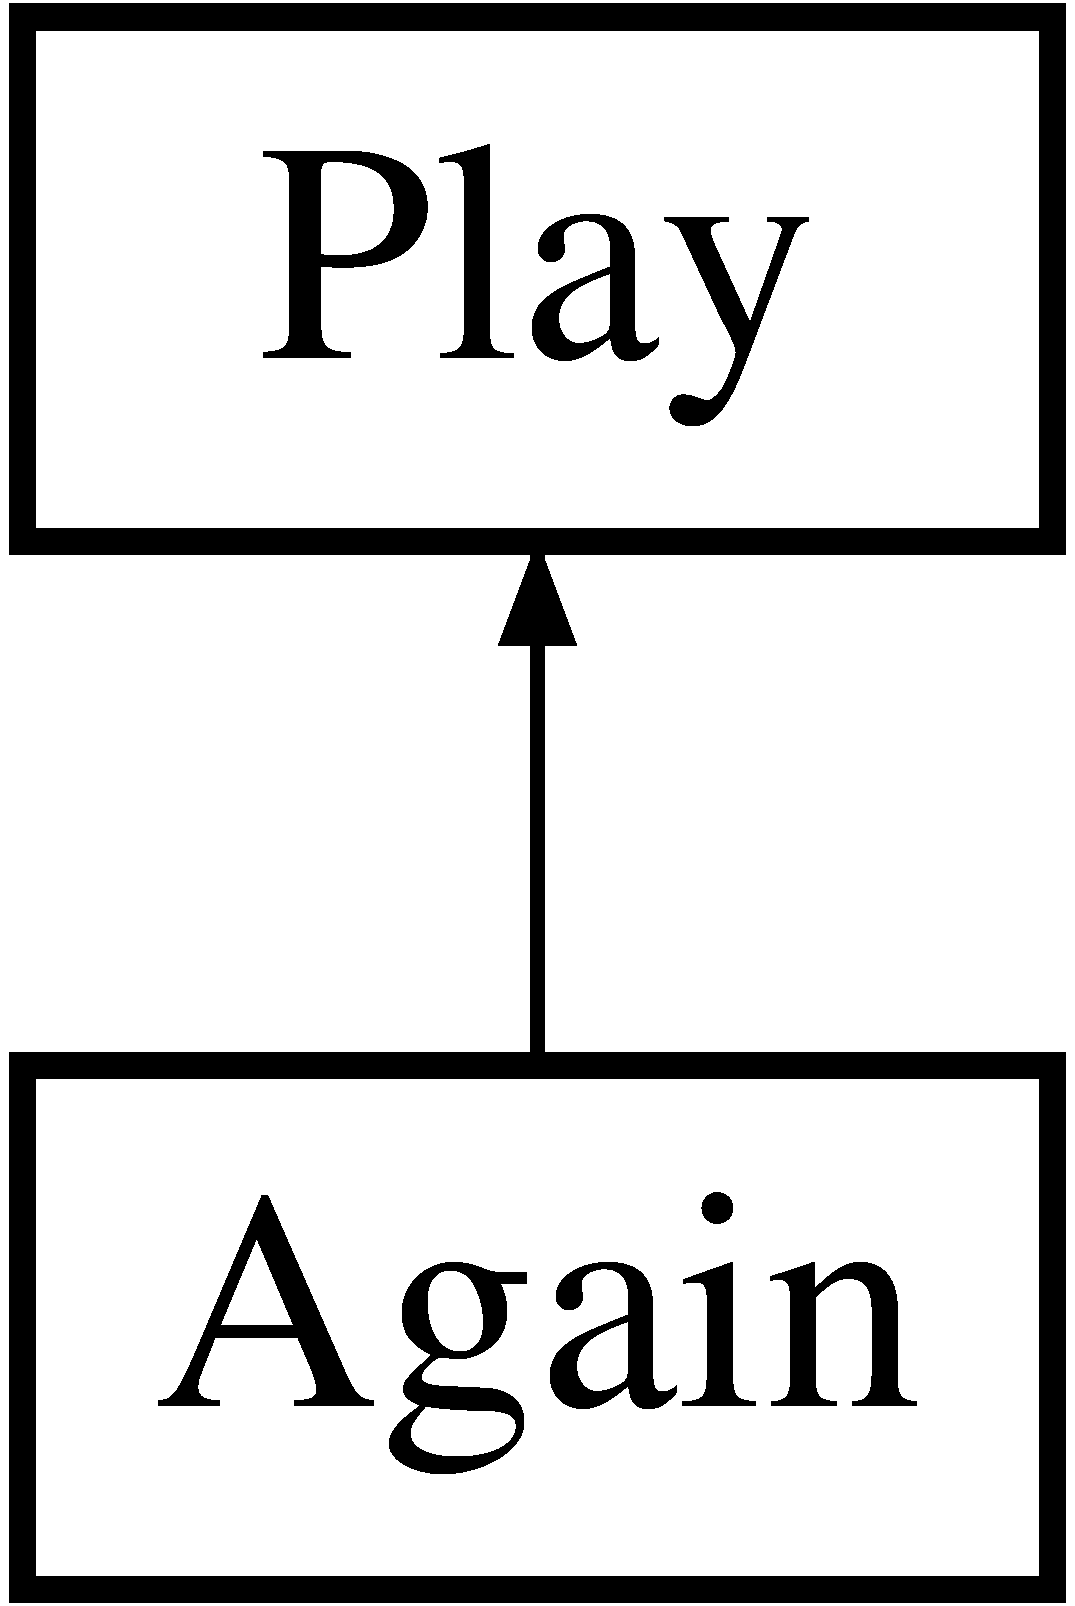
\includegraphics[height=2.000000cm]{class_play}
\end{center}
\end{figure}
\subsection*{Public Member Functions}
\begin{DoxyCompactItemize}
\item 
virtual void \hyperlink{class_play_a87bb5456a9fcecfb9075b73db83d1e4c}{show} ()
\end{DoxyCompactItemize}


\subsection{Detailed Description}


Definition at line 31 of file dornx2.\+h.



\subsection{Member Function Documentation}
\mbox{\Hypertarget{class_play_a87bb5456a9fcecfb9075b73db83d1e4c}\label{class_play_a87bb5456a9fcecfb9075b73db83d1e4c}} 
\index{Play@{Play}!show@{show}}
\index{show@{show}!Play@{Play}}
\subsubsection{\texorpdfstring{show()}{show()}}
{\footnotesize\ttfamily virtual void Play\+::show (\begin{DoxyParamCaption}{ }\end{DoxyParamCaption})\hspace{0.3cm}{\ttfamily [inline]}, {\ttfamily [virtual]}}



Reimplemented in \hyperlink{class_again_af3e99a5b59be21b644823ce7a9837a8f}{Again}.



Definition at line 33 of file dornx2.\+h.



The documentation for this class was generated from the following file\+:\begin{DoxyCompactItemize}
\item 
\hyperlink{dornx2_8h}{dornx2.\+h}\end{DoxyCompactItemize}

\chapter{File Documentation}
\hypertarget{_8dep_8inc}{}\section{.dep.\+inc File Reference}
\label{_8dep_8inc}\index{.\+dep.\+inc@{.\+dep.\+inc}}

\hypertarget{dornx2_8h}{}\section{dornx2.\+h File Reference}
\label{dornx2_8h}\index{dornx2.\+h@{dornx2.\+h}}
{\ttfamily \#include $<$iostream$>$}\newline
{\ttfamily \#include $<$string$>$}\newline
{\ttfamily \#include \char`\"{}dornx3.\+h\char`\"{}}\newline
\subsection*{Classes}
\begin{DoxyCompactItemize}
\item 
class \hyperlink{class_dornx2}{Dornx2}
\item 
class \hyperlink{class_play}{Play}
\item 
class \hyperlink{class_again}{Again}
\end{DoxyCompactItemize}
\subsection*{Functions}
\begin{DoxyCompactItemize}
\item 
{\footnotesize template$<$class T $>$ }\\T \hyperlink{dornx2_8h_a681e8a570f95d8ec2f9f2c05a9c603b0}{response} (T num)
\end{DoxyCompactItemize}


\subsection{Function Documentation}
\mbox{\Hypertarget{dornx2_8h_a681e8a570f95d8ec2f9f2c05a9c603b0}\label{dornx2_8h_a681e8a570f95d8ec2f9f2c05a9c603b0}} 
\index{dornx2.\+h@{dornx2.\+h}!response@{response}}
\index{response@{response}!dornx2.\+h@{dornx2.\+h}}
\subsubsection{\texorpdfstring{response()}{response()}}
{\footnotesize\ttfamily template$<$class T $>$ \\
T response (\begin{DoxyParamCaption}\item[{T}]{num }\end{DoxyParamCaption})}



Definition at line 46 of file dornx2.\+h.


\hypertarget{dornx2f_8cpp}{}\section{dornx2f.\+cpp File Reference}
\label{dornx2f_8cpp}\index{dornx2f.\+cpp@{dornx2f.\+cpp}}
{\ttfamily \#include $<$iostream$>$}\newline
{\ttfamily \#include $<$string$>$}\newline
{\ttfamily \#include $<$iomanip$>$}\newline
{\ttfamily \#include \char`\"{}dornx2.\+h\char`\"{}}\newline
\subsection*{Functions}
\begin{DoxyCompactItemize}
\item 
bool \hyperlink{dornx2f_8cpp_a7dd91336c52d1463f681f6252e3b91fa}{find\+Colo} (string c\mbox{[}$\,$\mbox{]}, int c\+Size, string test)
\end{DoxyCompactItemize}


\subsection{Function Documentation}
\mbox{\Hypertarget{dornx2f_8cpp_a7dd91336c52d1463f681f6252e3b91fa}\label{dornx2f_8cpp_a7dd91336c52d1463f681f6252e3b91fa}} 
\index{dornx2f.\+cpp@{dornx2f.\+cpp}!find\+Colo@{find\+Colo}}
\index{find\+Colo@{find\+Colo}!dornx2f.\+cpp@{dornx2f.\+cpp}}
\subsubsection{\texorpdfstring{find\+Colo()}{findColo()}}
{\footnotesize\ttfamily bool find\+Colo (\begin{DoxyParamCaption}\item[{string}]{c\mbox{[}$\,$\mbox{]},  }\item[{int}]{c\+Size,  }\item[{string}]{test }\end{DoxyParamCaption})}



Definition at line 15 of file dornx2f.\+cpp.


\hypertarget{dornx3_8h}{}\section{dornx3.\+h File Reference}
\label{dornx3_8h}\index{dornx3.\+h@{dornx3.\+h}}
{\ttfamily \#include $<$string$>$}\newline
\subsection*{Classes}
\begin{DoxyCompactItemize}
\item 
class \hyperlink{class_dornx3}{Dornx3}
\end{DoxyCompactItemize}
\subsection*{Variables}
\begin{DoxyCompactItemize}
\item 
const int \hyperlink{dornx3_8h_abbca5f70b1b16867a3fd2f340a1fbdd9}{S\+I\+Z\+E2} = 8
\item 
const int \hyperlink{dornx3_8h_afd1642892fe952b92046b3b290301c66}{C\+O\+L\+O\+R2} = 4
\end{DoxyCompactItemize}


\subsection{Variable Documentation}
\mbox{\Hypertarget{dornx3_8h_afd1642892fe952b92046b3b290301c66}\label{dornx3_8h_afd1642892fe952b92046b3b290301c66}} 
\index{dornx3.\+h@{dornx3.\+h}!C\+O\+L\+O\+R2@{C\+O\+L\+O\+R2}}
\index{C\+O\+L\+O\+R2@{C\+O\+L\+O\+R2}!dornx3.\+h@{dornx3.\+h}}
\subsubsection{\texorpdfstring{C\+O\+L\+O\+R2}{COLOR2}}
{\footnotesize\ttfamily const int C\+O\+L\+O\+R2 = 4}



Definition at line 15 of file dornx3.\+h.

\mbox{\Hypertarget{dornx3_8h_abbca5f70b1b16867a3fd2f340a1fbdd9}\label{dornx3_8h_abbca5f70b1b16867a3fd2f340a1fbdd9}} 
\index{dornx3.\+h@{dornx3.\+h}!S\+I\+Z\+E2@{S\+I\+Z\+E2}}
\index{S\+I\+Z\+E2@{S\+I\+Z\+E2}!dornx3.\+h@{dornx3.\+h}}
\subsubsection{\texorpdfstring{S\+I\+Z\+E2}{SIZE2}}
{\footnotesize\ttfamily const int S\+I\+Z\+E2 = 8}



Definition at line 14 of file dornx3.\+h.


\hypertarget{main_8cpp}{}\section{main.\+cpp File Reference}
\label{main_8cpp}\index{main.\+cpp@{main.\+cpp}}
{\ttfamily \#include $<$iostream$>$}\newline
{\ttfamily \#include $<$cstdlib$>$}\newline
{\ttfamily \#include $<$ctime$>$}\newline
{\ttfamily \#include $<$fstream$>$}\newline
{\ttfamily \#include $<$iomanip$>$}\newline
{\ttfamily \#include $<$string$>$}\newline
{\ttfamily \#include $<$vector$>$}\newline
{\ttfamily \#include \char`\"{}dornx2.\+h\char`\"{}}\newline
\subsection*{Classes}
\begin{DoxyCompactItemize}
\item 
struct \hyperlink{struct_inputs}{Inputs}
\end{DoxyCompactItemize}
\subsection*{Functions}
\begin{DoxyCompactItemize}
\item 
int \hyperlink{main_8cpp_a44e152a576d7364c9db95d5b8df6244c}{perc\+Res} (float, float)
\item 
void \hyperlink{main_8cpp_a7c0605d078db4fa9c78ebda0a2e9b043}{respond} (float)
\item 
bool \hyperlink{main_8cpp_acf4f606554ebcecbb158ee5e0d58dd57}{wnta} (float=0)
\item 
void \hyperlink{main_8cpp_aacf1e4e61cfe41a547ec5c5d780aa694}{dis\+Hi} ()
\item 
void \hyperlink{main_8cpp_abbb0723fc8e4be4a8f5412235c62a8b8}{get\+User} ()
\item 
bool \hyperlink{main_8cpp_ab72367d90929558eec111a464622f44d}{find\+Col} (string \mbox{[}$\,$\mbox{]}, int, string)
\item 
void \hyperlink{main_8cpp_a5f61db6c064bd1097f5e5d4ca6c660c7}{operator++} (string)
\item 
int \hyperlink{main_8cpp_a3c04138a5bfe5d72780bb7e82a18e627}{main} (int argc, char $\ast$$\ast$argv)
\end{DoxyCompactItemize}
\subsection*{Variables}
\begin{DoxyCompactItemize}
\item 
const int \hyperlink{main_8cpp_a99cb3c9797edb05222e1d4d9c8f9c03e}{P\+E\+R\+C\+E\+NT} =100
\item 
const int \hyperlink{main_8cpp_a2f3012b9ba71100daec1d9fecdf5b9ea}{H\+U\+N\+D\+R\+DS} =100
\item 
const int \hyperlink{main_8cpp_a64baef5dc7d1b0864a6a94f5d9cfb2fb}{T\+E\+NS} =10
\item 
const int \hyperlink{main_8cpp_afa42d960ad015515b6a28f1e22c7f4d0}{IN} = 1
\item 
const int \hyperlink{main_8cpp_af08413a3ee12cf78b0ddeea71e2648b3}{S\+I\+ZE} = 8
\item 
const int \hyperlink{main_8cpp_aa6d8034c897057de595a4511a4e7a837}{C\+O\+L\+OR} = 4
\item 
const int \hyperlink{main_8cpp_a449535d4215a26529b13febc509c199c}{S\+I\+Z\+E\+\_\+1} = 28
\item 
const int \hyperlink{main_8cpp_aef76f3385c12d0d696e38d02a917359f}{S\+I\+Z\+E\+\_\+2} = 29
\end{DoxyCompactItemize}


\subsection{Function Documentation}
\mbox{\Hypertarget{main_8cpp_aacf1e4e61cfe41a547ec5c5d780aa694}\label{main_8cpp_aacf1e4e61cfe41a547ec5c5d780aa694}} 
\index{main.\+cpp@{main.\+cpp}!dis\+Hi@{dis\+Hi}}
\index{dis\+Hi@{dis\+Hi}!main.\+cpp@{main.\+cpp}}
\subsubsection{\texorpdfstring{dis\+Hi()}{disHi()}}
{\footnotesize\ttfamily void dis\+Hi (\begin{DoxyParamCaption}{ }\end{DoxyParamCaption})}



Definition at line 235 of file main.\+cpp.

\mbox{\Hypertarget{main_8cpp_ab72367d90929558eec111a464622f44d}\label{main_8cpp_ab72367d90929558eec111a464622f44d}} 
\index{main.\+cpp@{main.\+cpp}!find\+Col@{find\+Col}}
\index{find\+Col@{find\+Col}!main.\+cpp@{main.\+cpp}}
\subsubsection{\texorpdfstring{find\+Col()}{findCol()}}
{\footnotesize\ttfamily bool find\+Col (\begin{DoxyParamCaption}\item[{string}]{c\mbox{[}$\,$\mbox{]},  }\item[{int}]{c\+Size,  }\item[{string}]{test }\end{DoxyParamCaption})}



Definition at line 293 of file main.\+cpp.

\mbox{\Hypertarget{main_8cpp_abbb0723fc8e4be4a8f5412235c62a8b8}\label{main_8cpp_abbb0723fc8e4be4a8f5412235c62a8b8}} 
\index{main.\+cpp@{main.\+cpp}!get\+User@{get\+User}}
\index{get\+User@{get\+User}!main.\+cpp@{main.\+cpp}}
\subsubsection{\texorpdfstring{get\+User()}{getUser()}}
{\footnotesize\ttfamily void get\+User (\begin{DoxyParamCaption}{ }\end{DoxyParamCaption})}



Definition at line 272 of file main.\+cpp.

\mbox{\Hypertarget{main_8cpp_a3c04138a5bfe5d72780bb7e82a18e627}\label{main_8cpp_a3c04138a5bfe5d72780bb7e82a18e627}} 
\index{main.\+cpp@{main.\+cpp}!main@{main}}
\index{main@{main}!main.\+cpp@{main.\+cpp}}
\subsubsection{\texorpdfstring{main()}{main()}}
{\footnotesize\ttfamily int main (\begin{DoxyParamCaption}\item[{int}]{argc,  }\item[{char $\ast$$\ast$}]{argv }\end{DoxyParamCaption})}



Definition at line 57 of file main.\+cpp.

\mbox{\Hypertarget{main_8cpp_a5f61db6c064bd1097f5e5d4ca6c660c7}\label{main_8cpp_a5f61db6c064bd1097f5e5d4ca6c660c7}} 
\index{main.\+cpp@{main.\+cpp}!operator++@{operator++}}
\index{operator++@{operator++}!main.\+cpp@{main.\+cpp}}
\subsubsection{\texorpdfstring{operator++()}{operator++()}}
{\footnotesize\ttfamily void operator++ (\begin{DoxyParamCaption}\item[{string}]{s }\end{DoxyParamCaption})}



Definition at line 301 of file main.\+cpp.

\mbox{\Hypertarget{main_8cpp_a44e152a576d7364c9db95d5b8df6244c}\label{main_8cpp_a44e152a576d7364c9db95d5b8df6244c}} 
\index{main.\+cpp@{main.\+cpp}!perc\+Res@{perc\+Res}}
\index{perc\+Res@{perc\+Res}!main.\+cpp@{main.\+cpp}}
\subsubsection{\texorpdfstring{perc\+Res()}{percRes()}}
{\footnotesize\ttfamily int perc\+Res (\begin{DoxyParamCaption}\item[{float}]{wl,  }\item[{float}]{n\+Games }\end{DoxyParamCaption})}



Definition at line 212 of file main.\+cpp.

\mbox{\Hypertarget{main_8cpp_a7c0605d078db4fa9c78ebda0a2e9b043}\label{main_8cpp_a7c0605d078db4fa9c78ebda0a2e9b043}} 
\index{main.\+cpp@{main.\+cpp}!respond@{respond}}
\index{respond@{respond}!main.\+cpp@{main.\+cpp}}
\subsubsection{\texorpdfstring{respond()}{respond()}}
{\footnotesize\ttfamily void respond (\begin{DoxyParamCaption}\item[{float}]{n }\end{DoxyParamCaption})}



Definition at line 216 of file main.\+cpp.

\mbox{\Hypertarget{main_8cpp_acf4f606554ebcecbb158ee5e0d58dd57}\label{main_8cpp_acf4f606554ebcecbb158ee5e0d58dd57}} 
\index{main.\+cpp@{main.\+cpp}!wnta@{wnta}}
\index{wnta@{wnta}!main.\+cpp@{main.\+cpp}}
\subsubsection{\texorpdfstring{wnta()}{wnta()}}
{\footnotesize\ttfamily bool wnta (\begin{DoxyParamCaption}\item[{float}]{n = {\ttfamily 0} }\end{DoxyParamCaption})}



Definition at line 228 of file main.\+cpp.



\subsection{Variable Documentation}
\mbox{\Hypertarget{main_8cpp_aa6d8034c897057de595a4511a4e7a837}\label{main_8cpp_aa6d8034c897057de595a4511a4e7a837}} 
\index{main.\+cpp@{main.\+cpp}!C\+O\+L\+OR@{C\+O\+L\+OR}}
\index{C\+O\+L\+OR@{C\+O\+L\+OR}!main.\+cpp@{main.\+cpp}}
\subsubsection{\texorpdfstring{C\+O\+L\+OR}{COLOR}}
{\footnotesize\ttfamily const int C\+O\+L\+OR = 4}



Definition at line 27 of file main.\+cpp.

\mbox{\Hypertarget{main_8cpp_a2f3012b9ba71100daec1d9fecdf5b9ea}\label{main_8cpp_a2f3012b9ba71100daec1d9fecdf5b9ea}} 
\index{main.\+cpp@{main.\+cpp}!H\+U\+N\+D\+R\+DS@{H\+U\+N\+D\+R\+DS}}
\index{H\+U\+N\+D\+R\+DS@{H\+U\+N\+D\+R\+DS}!main.\+cpp@{main.\+cpp}}
\subsubsection{\texorpdfstring{H\+U\+N\+D\+R\+DS}{HUNDRDS}}
{\footnotesize\ttfamily const int H\+U\+N\+D\+R\+DS =100}



Definition at line 22 of file main.\+cpp.

\mbox{\Hypertarget{main_8cpp_afa42d960ad015515b6a28f1e22c7f4d0}\label{main_8cpp_afa42d960ad015515b6a28f1e22c7f4d0}} 
\index{main.\+cpp@{main.\+cpp}!IN@{IN}}
\index{IN@{IN}!main.\+cpp@{main.\+cpp}}
\subsubsection{\texorpdfstring{IN}{IN}}
{\footnotesize\ttfamily const int IN = 1}



Definition at line 25 of file main.\+cpp.

\mbox{\Hypertarget{main_8cpp_a99cb3c9797edb05222e1d4d9c8f9c03e}\label{main_8cpp_a99cb3c9797edb05222e1d4d9c8f9c03e}} 
\index{main.\+cpp@{main.\+cpp}!P\+E\+R\+C\+E\+NT@{P\+E\+R\+C\+E\+NT}}
\index{P\+E\+R\+C\+E\+NT@{P\+E\+R\+C\+E\+NT}!main.\+cpp@{main.\+cpp}}
\subsubsection{\texorpdfstring{P\+E\+R\+C\+E\+NT}{PERCENT}}
{\footnotesize\ttfamily const int P\+E\+R\+C\+E\+NT =100}



Definition at line 21 of file main.\+cpp.

\mbox{\Hypertarget{main_8cpp_af08413a3ee12cf78b0ddeea71e2648b3}\label{main_8cpp_af08413a3ee12cf78b0ddeea71e2648b3}} 
\index{main.\+cpp@{main.\+cpp}!S\+I\+ZE@{S\+I\+ZE}}
\index{S\+I\+ZE@{S\+I\+ZE}!main.\+cpp@{main.\+cpp}}
\subsubsection{\texorpdfstring{S\+I\+ZE}{SIZE}}
{\footnotesize\ttfamily const int S\+I\+ZE = 8}



Definition at line 26 of file main.\+cpp.

\mbox{\Hypertarget{main_8cpp_a449535d4215a26529b13febc509c199c}\label{main_8cpp_a449535d4215a26529b13febc509c199c}} 
\index{main.\+cpp@{main.\+cpp}!S\+I\+Z\+E\+\_\+1@{S\+I\+Z\+E\+\_\+1}}
\index{S\+I\+Z\+E\+\_\+1@{S\+I\+Z\+E\+\_\+1}!main.\+cpp@{main.\+cpp}}
\subsubsection{\texorpdfstring{S\+I\+Z\+E\+\_\+1}{SIZE\_1}}
{\footnotesize\ttfamily const int S\+I\+Z\+E\+\_\+1 = 28}



Definition at line 28 of file main.\+cpp.

\mbox{\Hypertarget{main_8cpp_aef76f3385c12d0d696e38d02a917359f}\label{main_8cpp_aef76f3385c12d0d696e38d02a917359f}} 
\index{main.\+cpp@{main.\+cpp}!S\+I\+Z\+E\+\_\+2@{S\+I\+Z\+E\+\_\+2}}
\index{S\+I\+Z\+E\+\_\+2@{S\+I\+Z\+E\+\_\+2}!main.\+cpp@{main.\+cpp}}
\subsubsection{\texorpdfstring{S\+I\+Z\+E\+\_\+2}{SIZE\_2}}
{\footnotesize\ttfamily const int S\+I\+Z\+E\+\_\+2 = 29}



Definition at line 29 of file main.\+cpp.

\mbox{\Hypertarget{main_8cpp_a64baef5dc7d1b0864a6a94f5d9cfb2fb}\label{main_8cpp_a64baef5dc7d1b0864a6a94f5d9cfb2fb}} 
\index{main.\+cpp@{main.\+cpp}!T\+E\+NS@{T\+E\+NS}}
\index{T\+E\+NS@{T\+E\+NS}!main.\+cpp@{main.\+cpp}}
\subsubsection{\texorpdfstring{T\+E\+NS}{TENS}}
{\footnotesize\ttfamily const int T\+E\+NS =10}



Definition at line 23 of file main.\+cpp.


%--- End generated contents ---

% Index
\backmatter
\newpage
\phantomsection
\clearemptydoublepage
\addcontentsline{toc}{chapter}{Index}
\printindex

\end{document}
